\documentclass{article}
\usepackage[utf8]{inputenc}
\usepackage{graphicx}
\usepackage{tikz}
\usepackage[most]{tcolorbox}
\usepackage[top=2cm, bottom=2cm, outer=0cm, inner=0cm]{geometry}

\begin{document}

\tikz[remember picture,overlay] \node[opacity=0.3,inner sep=0pt] at (current page.center){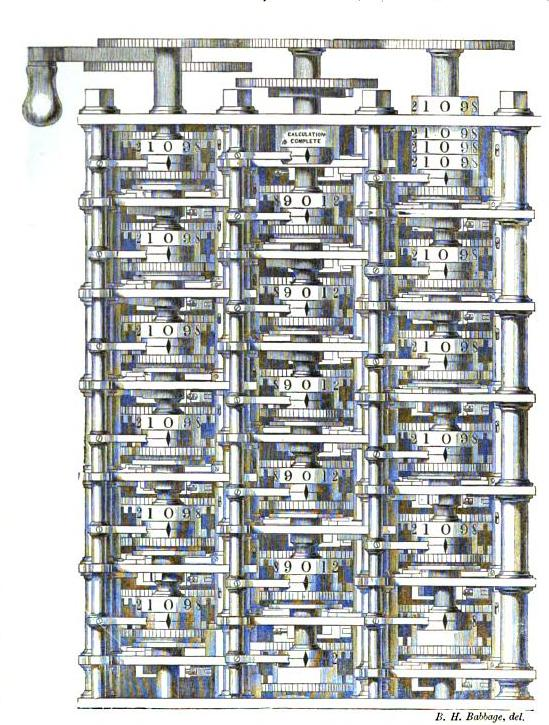
\includegraphics[width=\paperwidth,height=\paperheight]{./comp.jpg}};

\begin{centering}
  
\includegraphics[width=0.9\textwidth]{./header.jpg}
  \\
  \begin{tcolorbox}[enhanced jigsaw,
                  colback=gray!30,%gray background
                  width=0.8\linewidth,% Use 5cm total width,
                  arc=3mm, auto outer arc,
                  boxrule=5pt
                 ]
      {\bf Bingoregler:} Målet är att under paneldiskussionen samla så många bingorader (horisontellt, vertikalt och diagonalt) som möjligt genom att lyssna uppmärksamt och kryssa i rutorna för de AI-klichéer som används. Icke-strikt semantisk likhet räknas, det vill säga ``universell basinkomst'' och ``medborgarlön'' kan ses som synonymer.

   
  \end{tcolorbox}
\end{centering}
\end{document}
